\documentclass[10pt]{extarticle}
\title{}
\author{Avinash Iyer}
\date{}
\usepackage[shortlabels]{enumitem}

%font setup
%
%\usepackage[math]{anttor}

%paper setup
\usepackage{geometry}
\geometry{letterpaper, portrait, margin=1in}
\usepackage{fancyhdr}

%symbols
\usepackage{amsmath}
\usepackage{amssymb}
\usepackage{hyperref}
\usepackage{gensymb}

\usepackage[T1]{fontenc}
\usepackage[utf8]{inputenc}

%chemistry stuff
\usepackage[version=4]{mhchem}
\usepackage{chemfig}

%plotting
\usepackage{pgfplots}
\usepackage{tikz}

%\usepackage{natbib}

%graphics stuff
\usepackage{graphicx}
\graphicspath{ {./images/} }

%code stuff
%when using minted, make sure to add the -shell-escape flag
%you can use lstlisting if you don't want to use minted
%\usepackage{minted}
%\usemintedstyle{pastie}
%\newminted[javacode]{java}{frame=lines,framesep=2mm,linenos=true,fontsize=\footnotesize,tabsize=3,autogobble,}
%\newminted[cppcode]{cpp}{frame=lines,framesep=2mm,linenos=true,fontsize=\footnotesize,tabsize=3,autogobble,}

\usepackage{listings}
\usepackage{color}
\definecolor{dkgreen}{rgb}{0,0.6,0}
\definecolor{gray}{rgb}{0.5,0.5,0.5}
\definecolor{mauve}{rgb}{0.58,0,0.82}

\lstset{frame=tb,
	language=Java,
	aboveskip=3mm,
	belowskip=3mm,
	showstringspaces=false,
	columns=flexible,
	basicstyle={\small\ttfamily},
	numbers=none,
	numberstyle=\tiny\color{gray},
	keywordstyle=\color{blue},
	commentstyle=\color{dkgreen},
	stringstyle=\color{mauve},
	breaklines=true,
	breakatwhitespace=true,
	tabsize=3
}
% text + color boxes
\usepackage{tcolorbox}
\tcbuselibrary{breakable}
\newtcolorbox{problem}[1]{colback = white, title = {#1}, breakable}
\newtcolorbox{solution}{colback = white, colframe = black!75!white, title = Solution}
%including PDFs
\usepackage{pdfpages}
\setlength{\parindent}{0pt}

\pagestyle{fancy}
\fancyhf{}
\rhead{Avinash Iyer}
\lhead{Midterm 1 Review}
\begin{document}
  \section*{1.1}
  \begin{problem}{Basics}
  A \textbf{graph} is a collection of vertices and edges with a given relation denoted $G = (V,E,R)$. Most of the time, we just use $G$ to denote the entirety of $(V,E,R)$. A graph is \textbf{simple} if there is only one edge between two vertices, and there are no loops (i.e., an edge that connects a vertex to itself). We will be dealing with simple graphs for now.\\

  Edges between two vertices $u$ and $v$ are denoted $uv$, and this edge is \textbf{incident} on two vertices. Two vertices are \textbf{adjacent} if there exists an edge between them. Adjacency is denoted $u\leftrightarrow v$.\\

  Two graphs are equal of $E(G) = E(H)$ and $V(G) = V(H)$, while they're isomorphic if $\exists \varphi: G\rightarrow H$ such that $uv\in E(G) \leftrightarrow \varphi(u)\varphi(v)\in E(H)$ where $\varphi$ is a bijection. This is similar to the definition of isomorphisms for groups and rings. An isomorphism class is the equivalence class of graphs under the isomorphism relation (this is akin to a graph without labeled vertices). \\
  \end{problem}
\begin{problem}{Complete Graphs and Subgraphs}
  \textbf{Complete} graphs are ones where every vertex has an edge to every other vertex. They are denoted $K_n$. An example of $K_4$ is shown below.
  \begin{center}
    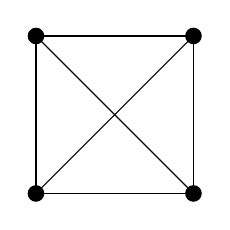
\begin{tikzpicture}
      \fill (1,1) circle (3pt);
      \fill (-1,1) circle (3pt);
      \fill (1,-1) circle (3pt);
      \fill (-1,-1) circle (3pt);
      \draw (1,1) -- (1,-1) -- (-1,-1) -- (-1,1) -- (1,1);
      \draw (1,1) -- (-1,-1);
      \draw (1,-1) -- (-1,1);
    \end{tikzpicture}
  \end{center}
  A \textbf{subgraph} is a graph $H$ such that $V(H) \subseteq V(G)$ and $E(H) \subseteq E(G)$. For example, the following is a subgraph of $K_4$
  \begin{center}
    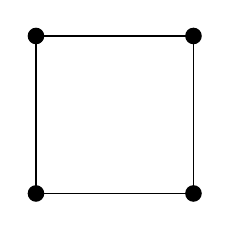
\begin{tikzpicture}
      \fill (1,1) circle (3pt);
      \fill (-1,1) circle (3pt);
      \fill (1,-1) circle (3pt);
      \fill (-1,-1) circle (3pt);
      \draw (1,1) -- (1,-1) -- (-1,-1) -- (-1,1) -- (1,1);
    \end{tikzpicture}
  \end{center}
  An \textbf{induced subgraph} is a subgraph such that $E(H)$ is the set of all edges in $G$ that connects vertices in $V(H)$. It is usually denoted $G[V(H)]$. For example, we can see an induced subgraph in $K_4$ selecting three vertices as follows:
  \begin{center}
    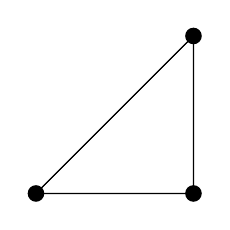
\begin{tikzpicture}
      \fill (1,1) circle (3pt);
      \fill (1,-1) circle (3pt);
      \fill (-1,-1) circle (3pt);
      \draw (1,1) -- (1,-1) -- (-1,-1) -- (1,1);
      \draw (1,1) -- (-1,-1);
    \end{tikzpicture}
  \end{center}
\end{problem}
\begin{problem}{Paths, Cycles, and Complements}
  A \textbf{path} is a nonempty graph in the form $P = x_1,x_2,\dots,x_k$ with edge set $E(P) = \{x_1x_2, x_2x_3,\dots,x_{k-1}x_k\}$, where edges don't repeat themselves. A cycle is a path where we include the edge $x_kx_1$. We will learn about different kinds of paths, trails, etc. in section 1.2.\\

  The complement of a graph, $\overline{G}$ is found by using the same vertex set and taking the complement of the edge set. In other words, $V(\overline{G}) = V(G)$ and $E(\overline{G}) = \overline{E(G)}$. For example, we can consider the complete bipartite graph $K_{3,3}$ (explained later), and see its complement.
  \begin{center}
    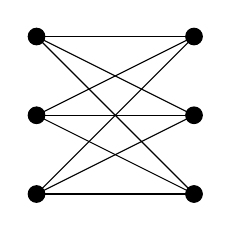
\begin{tikzpicture}
      \filldraw (-1,1) circle (3pt)
                (-1,0) circle (3pt)
                (-1,-1) circle (3pt)
                (1,-1) circle (3pt)
                (1,0) circle (3pt)
                (1,1) circle (3pt);
      \draw (-1,1) -- (1,1);
      \draw (-1,1) -- (1,0);
      \draw (-1,1) -- (1,-1);
      \draw (-1,-1) -- (1,1);
      \draw (-1,-1) -- (1,0);
      \draw (-1,-1) -- (1,-1);
      \draw (-1,0) -- (1,1);
      \draw (-1,0) -- (1,0);
      \draw (-1,0) -- (1,-1);
    \end{tikzpicture}
  \end{center}
  \begin{center}
    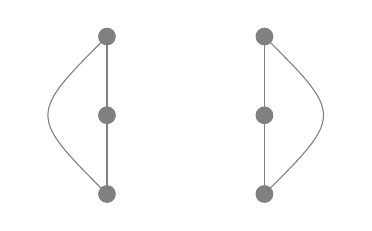
\begin{tikzpicture}
      \filldraw[gray] (-1,1) circle (3pt)
                (-1,0) circle (3pt)
                (-1,-1) circle (3pt)
                (1,-1) circle (3pt)
                (1,0) circle (3pt)
                (1,1) circle (3pt);
    \draw[gray] (-1,1) -- (-1,0) -- (-1,-1);
    \draw[gray] (-1,-1) .. controls (-2,0) .. (-1,1);
    \draw[gray] (1,1) -- (1,0) -- (1,-1);
    \draw[gray] (1,-1) .. controls (2,0) .. (1,1);
    \end{tikzpicture}
  \end{center}
  We can see that the complement is isomorphic to two copies of $K_3$, which is the triangle graph.\\

  A \textbf{independent set} is a set of vertices that are not adjacent to each other in $G$ (implying they are adjacent to each other in $\overline{G}$). For example, the independent sets in the above graph of $K_{3,3}$ are those two sets of $K_3$. The independence number $\alpha(G)$ is the cardinality of the largest independent set in $G$.\\

  Similarly, a complete subgraph, also known as a \textbf{clique} is a subgraph of $G$ where all the vertices are connected to every other vertex, implying that the clique is an independent set in $\overline{G}$. The clique number, $\omega(G)$ is the size of the largest clique. We can see that $\omega(G) = \alpha(\overline{G})$ and vice versa.
\end{problem}
\begin{problem}{Partitions}
  A graph is \textbf{bipartite} if there exists a partition $G = X\sqcup Y$ (where $\sqcup$ denotes the disjoint union) where $X$ and $Y$ are independent sets. A bipartite graph is \textbf{complete} if $\forall x\in X, \forall y\in Y, x\leftrightarrow y$. Complete bipartite graphs are denoted $K_{m,n}$, where $m$ denotes the size of one independent set and $n$ denotes the size of the other independent set.\\

  Similarly, a $k$-partite graph is one where $G = V_1\sqcup V_2\sqcup \cdots \sqcup V_k$, where $V_i$ is an independent set for all $1\leq i\leq k$. A $k$-partite graph is complete if every vertex in $V_i$ is adjacent to every other vertex in every other $V_i$.\\

  A \textbf{coloring} of a graph is a function $f: V\rightarrow S$ such that $f(v) \neq f(w)$ if $v\leftrightarrow w$. A bipartite graph is 2-colorable, and a graph is $k$-partite if and only if it is $k$-colorable.\\
\end{problem}
\begin{problem}{Matrices}
  The \textbf{adjacency matrix} of a graph is a matrix defined as follows:
  \[
    A(v,e) = \begin{cases}
      1\textrm{ if } v\in e\\
      0\textrm{ if } v\notin e
    \end{cases}
  \]
  The incidence matrix, on the other hand, represents the vertices on the rows and the edges on the columns --- for a given row, a $1$ is placed in a column for any edge the vertex is incident on. We can show that $A^2 = MM^T$ for adjacency matrix $A$ and incidence matrix $M$ for any given graph. The incidence matrix need not be square, but the adjacency matrix is necessarily square

  \begin{itemize}
    \item The sum of any given row in the incidence matrix is the number of edges incident with the vertex, or $d(v)$ (for degree).
    \item The sum any given column in the incidence matrix is $2$, for a simple graph.
    \item The sum of any given row or column in $A$ is the number of vertices adjacent to the vertex, once again yielding $d(v)$.
    \item We can show that $A^2 = MM^T$ for adjacency matrix $A$ and incidence matrix $M$ on any given graph.
  \end{itemize}
\end{problem}
\begin{problem}{The Petersen Graph}
  We can also examine combinatorial relations through graphs. For example, the Petersen graph ($G_p$) is defined as follows:
  \begin{quote}
    The simple graph whose vertices are the 2-element subsets of a 5 element set, and whose edges are the pairs of disjoint 2-element sets.
  \end{quote}
  \begin{center}
    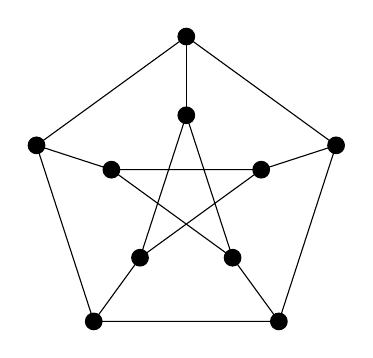
\begin{tikzpicture}
      \draw (18:2cm) -- (90:2cm) -- (162:2cm) -- (234:2cm) --
      (306:2cm) -- cycle;
      \draw (18:1cm) -- (162:1cm) -- (306:1cm) -- (90:1cm) --
      (234:1cm) -- cycle;
      \foreach \x in {18,90,162,234,306}{
      \draw (\x:1cm) -- (\x:2cm);
      \filldraw (\x:2cm) circle (3pt);
      \filldraw (\x:1cm) circle (3pt);
      }
    \end{tikzpicture}
  \end{center}
  We can show a couple theorems using this definition of the Petersen Graph.
  \begin{problem}{Propositions about the Petersen Graph}
    \begin{itemize}
      \item Every vertex in the Petersen graph has degree 3.
      \item If two vertices are non-adjacent in the Petersen graph, they share exactly one common neighbor.
      \item The girth (or length of the shortest cycle) of the Petersen graph is $5$.
    \end{itemize}
  \end{problem}
  \begin{problem}{Solution}
    Because there are $3$ elements in $[5] = \{1,2,3,4,5\}$ not equal to any given set of two numbers, we know that the number of vertices adjacent to any given element is $\begin{pmatrix} 3\\ 2\end{pmatrix} = 3$.\\ 

    Suppose two elements $v_1\neq v_2$ are in $V(G_p)$ where $v_1\not\leftrightarrow v_2$. Then, it must be the case that $v_1\cap v_2\neq 0$, meaning that $|v_1\cap v_2| = 1$, and $|v_1\cup v_2| = 3$, implying that $|[5] - v_1\cup v_2| = 2$. There is only one $v_k\in V(G_p)$ such that $v_k$ has two elements, defined as $v_k = [5] - (v_1\cup v_2)$.\\

    Suppose $G_p$ has a cycle of length $3$. Since a cycle of $3$ would be isomorphic to $K_3$, this means there are three disjoint vertices $v_1,v_2,v_3\in V(G)$, implying that $|v_1 \cup v_2 \cup v_3| = |v_1| + |v_2| + |v_3| = 6$. However, the original set has cardinality $5$. Suppose there were a $4$-cycle --- this would mean that two vertices share a common neighbor, which we previously showed was not possible in $G_p$.
  \end{problem}
\end{problem}
\begin{problem}{Decompositions}
  A \textbf{decomposition} is a list of subgraphs of a graph such that every \textit{edge} appears only once (vertices are allowed to repeat themselves).

  A graph is \textbf{self-complementary} if it is isomorphic (not equal) to its complement. An $n$-vertex graph, $H$, is self-complementary if and only if $K_n$ has a decomposition consisting of two copies of $H$.\\

  \begin{itemize}
    \item $C_5$ is self-complementary because $K_5$ can be decomposed into two copies of $C_5$.
    \item $K_4$ can be decomposed into three copies of $P_3$.
    \item $K_{3,3}$ can be decomposed into three sets of pairwise disjoint matchings (where a matching denotes a set of disjoint edges that share no common vertex).
    \item A $k$-regular bipartite graph (this will be discussed in section 1.3) will have $k$ perfect matchings.
  \end{itemize}
\end{problem}
\section*{1.2}%
\begin{problem}{Walks, Trails, and Paths}
  A \textbf{walk} is a series of alternating vertices and edges $v_0e_0v_1e_1\cdots e_{k-1}v_k$. The vertices and edges in a walk can repeat themselves --- if a graph is simple, all you need do is list the vertices of a walk.\\

  If $v_0 = v_k$, the walk is closed, else it is an open walk, and the length of the walk is equal to the number of \textit{edges} in the walk.\\

  A \textbf{trail} is a walk that does not repeat edges, while a \textbf{circuit} is a closed trail. Circuits are usually written in cyclic order, but there is not necessarily any starting or ending point of a circuit.\\

  A \textbf{path} is a walk that does not repeat vertices or edges, and a cycle is a circuit that does not repeat vertices.\\

  We can prove the following proposition:
  \begin{problem}{Proposition}
    Every $u,v$ walk contains a $u,v$ path.
  \end{problem}
  \begin{problem}{Solution}
    Let $u,\dots,x,\dots,x,\dots,v$ be a path. If there exists copies of any vertex $x$, delete all edges and vertices between instances of $x$ and retain one of the instances of $x$, along with the remaining edges. Continue until there are no repeated instances of any vertices.
  \end{problem}
\end{problem}
\begin{problem}{Components and Connections}
  A graph is \textbf{connected} if $\forall x,y\in G$, $\exists x,y$ path. Notice that we said \textit{path}, not necessarily adjacent --- obviously if $x\leftrightarrow y$, they have a path between them, but adjacency is not enough to show connectedness.\\

  A \textbf{component} is a maximal connected subgraph of any graph.
  \begin{problem}{Maximal vs. Maximum}
    ``Maximum'' simply describes the largest set that satisfies the property --- for example, if we had a graph where one subgraph was $K_4$ and there were no subgraphs that were larger than $K_4$, we would say that particular subgraph was a \textit{maximum} clique.\\

    Meanwhile, ``maximal'' describes a property where adding an additional vertex or edge would violate the property. For example, imagine a graph that were $K_4$ with one vertex adjacent to a vertex that was also adjacent to $K_5$. If we started describing $K_4$, we would reach a point where adding an additional vertex would make the graph no longer complete --- thus, $K_4$ is a \textit{maximal} clique.\\

    Important for us is that a \textbf{maximal path} is one that cannot be extended. This will help us in various proofs later on.
  \end{problem}
  The relation $uRv$ if and only if there is a $u,v$ path in $G$ is known as the \textbf{connection relation}, and it is an equivalence relation (reflexive, symmetric, and transitive). The equivalence classes of the connection relation are the components of $G$.
\end{problem}
\begin{problem}{Edge and Vertex Deletions}
  If $U\subseteq V(G)$, then $G-U$ is equal to deleting all the vertices in $U$ and the edges incident on the vertices in $U$, or $G[V-U]$. If $U = \{v\}$, then we denote it $G-v$. An edge deletion doesn't require deleting the vertices the edge is incident on.\\

  By adding an edge to a graph, we either leave the number of components unchanged or increase them by one, which implies the following proposition.
  \begin{problem}{Proposition}
    Every graph with $n$ vertices and $k$ edges has at least $n-k$ components.
  \end{problem}
  \begin{problem}{Proof}
    Start with $n$ vertices and $0$ edges. There are $n$ components in this graph --- by adding an edge, we decrease the number of components by $1$ or leave them unchanged, thus yielding us that the number of components is at least $n-k$.
  \end{problem}
  A \textbf{cut-edge} or \textbf{cut-vertex} is an edge or vertex whose deletion increases the number of components in $G-e$ or $G-v$. We can prove the following proposition:
  \begin{problem}{Proposition}
    An edge is a cut-edge if and only if it is not contained within a cycle.
  \end{problem}
  \begin{problem}{Proof}
    This is equivalent to saying that for some connected graph $H$, $H-e$ is connected if and only if $e$ is in a cycle in $H$.\\

    Suppose $H-e$ is connected. Then, there must exist a path $P$ in $H-e$ such that $P+e$ is a cycle.\\

    Suppose that $e$ is in a cycle in $H$. Since $H$ is connected, then $\exists u,v$ path $P$ in $H$. We then get the two following cases:
    \begin{itemize}
      \item If $e\notin P$, then $P\in H-e$, so $H-e$ is connected.
      \item If $e\in P$, then without loss of generality, the vertex $x$ appears before the vertex $y$, and that $e = xy$. We can construct a $u,v$ path as follows: $P = u,\dots,x,y,\dots, v$ in $H$. Since $e$ is in cycle $C$, we can create a $u,v$ walk in $H-e$ as follows:
        \begin{itemize}
          \item Follow $P$ from $u$ to $x$
          \item Follow $C-e$ from $x$ to $y$
          \item Follow $P$ from $y$ to $v$
        \end{itemize}
      \item Since every $u,v$ walk contains a $u,v$ path, we have showed that $\exists u,v$ path in $H-e$, so $H-e$ is connected.
    \end{itemize}
  \end{problem}
\end{problem}
\begin{problem}{Even and Odd Walks}
  A walk is \textbf{even} if it is of even length (as denoted by the number of edges), and a walk is \textbf{odd} if it is of odd length. Every closed walk $W$ contains a cycle $C$ if the vertices and edges of $C$ occur in cyclic order as a sublist of $W$.
  \begin{problem}{Proposition}
    Every closed odd walk contains an odd cycle.
  \end{problem}
  \begin{problem}{Proof}
    We will proceed via induction as follows:
    \begin{description}[font=\normalfont\scshape]
      \item[Base Case] If $\ell = 1$, then we know that this is a cycle.
      \item [Inductive Hypothesis] Find a repeated vertex $x$ within $W$ aside from the starting point $u$ itself. That is, $W = u,\dots,x,\dots,x,\dots,u$. If there is no repeated vertex other than $u$ itself, then we have an odd cycle.
      \item[Proof] Else, consider $W' = x,\dots,x$ and $W'' = u,\dots,x,\dots,u$ found by deleting the first instance of $x$ and the remaining edges between that first instance and the second instance of $x$. We know that since $\ell(W)$ is odd, and $\ell(W) = \ell(W') + \ell(W'')$, we must have that one of $\ell(W')$ or $\ell(W'')$ must be odd.
    \end{description}
  \end{problem}
  \begin{problem}{Proposition}
    If an edge appears exactly once in a closed walk $W$, then $W$ contains a cycle through that edge, $e$.
  \end{problem}
  \begin{problem}{Proof}
    Without loss of generality, let $W = y,\dots,x,y$, and $e = xy$. Then, $W' = y,\dots,x$ is a $y,x$ walk, implying $\exists y,x$ path $P$. Therefore, $P + e$ yields a cycle.
  \end{problem}
  \begin{problem}{König's Theorem}
    A graph is bipartite if and only if it does not contain an odd cycle.
  \end{problem}
  In order to prove something \textit{is} bipartite, it is easier to find a bipartition than to show that all cycles in the graph are even.
  \begin{problem}{Proof}
    Let $\textrm{dist}(x,y)$ denote the length of the shortest path between $x$ and $y$, and let $G$ be a connected graph. Let $v\in V(G)$ and $X = \{v\in V(G): \textrm{dist}(v,x)\textrm{ is even} \}$, and $Y = \{v\in V(G): \textrm{dist}(v,x)\textrm{ is odd} \}$, where $x$ is some vertex. Assume towards contradiction that one of either $X$ or $Y$ is not an independent set. Without loss of generality, let $X$ be the set that is not independent. Let $e = x_1x_2$ be an edge for some $x_1,x_2\in X$. Then, we can construct a path as follows:
    \begin{itemize}
      \item $P_1 = v,\dots,x_1$
      \item $e = x_1x_2$
      \item $P_2 = x_2,\dots,v_2$
    \end{itemize}
    ($\Rightarrow$) By our definition, we know that $P_1$ and $P_2$ are even, and that $C = P_1 + e + P_2$ is an odd cycle. Therefore, we have shown that every graph that is not bipartite contains an odd cycle.\\
    
    ($\Leftarrow$) We can show that every bipartite graph contains an odd cycle since every walk that starts in one independent set $X$ that ends in the independent set $X$ must have even parity. Therefore, all cycles in a bipartite graph must be even.
  \end{problem}
\end{problem}
\begin{problem}{Graph Unions}
  The union of a set of graphs $G_1,\dots,G_k$ is defined as follows:
  \[
    V = \bigcup_{i = 1}^{k} V(G_i)~ E = \bigcup_{i = 1}^{k} E(G_i)
  \]
  Each edge in $G$ can be contained within more than one graph in a graph union, but that is not the case for a graph decomposition.\\

  For example, $K_4 = C_4 \cup C_4$. but $K_4$ does not decompose into two copies of $C_4$ since it only contains six edges.
\end{problem}
\begin{problem}{Eulerian Graphs}
  A graph $G$ is \textbf{Eulerian} if it contains a circuit that contains all the edges in $G$, known as an Eulerian circuit. Vertices may repeat themselves, but edges may not.\\
  \begin{problem}{Lemma}
    If $\forall v\in G$, $d(v) \geq 2$, then $G$ contains a cycle.
  \end{problem}
  \begin{problem}{Proof}
    Let $P = u_1,u_2,\dots,u_k$ be a maximal path. Since $d(u_1)\geq 2$ by our assumption, this means $u_1$ is incident on some edge other than $u_1u_2$. However, since $P$ is maximal and cannot be extended, this means $u_1$ must be incident on an edge that is also incident on $v\in \{u_1,\dots,u_k\}$, implying the existence of a cycle $C = u_1,v,\dots,u_2,u_1$.
  \end{problem}
  Using this lemma, we can prove the following important result about Eulerian graphs:
  \begin{problem}{Proposition}
    A graph is Eulerian if and only if it has at most one nontrivial component and all vertices are of even degree.
  \end{problem}
  \begin{problem}{Proof}
    ($\Rightarrow$) Whenever we ``enter'' a vertex during an Eulerian circuit, we also have to ``exit'' the vertex at an edge. If a vertex is not on the trail, then it has no incident edges and so the vertex is a trivial component. Additionally, if $G$ has multiple components, then there is no trail connecting all components and so $G$ cannot be Eulerian.\\

    ($\Leftarrow$) Suppose all vertices of $G$ are of even degree and $G$ has only one nontrivial component. Let $e(G) = |E(G)|$
    \begin{description}[font=\normalfont\scshape]
      \item[Base Case] Suppose $e(G) = 0$. Then, there is an Eulerian circuit and every vertex is of even degree (namely, $0$).
      \item[Inductive Hypothesis] If $e(G) > 0$, then every vertex in $G$ has a degree at least $2$. This means $\exists C\subseteq G$ where $C$ is a cycle. If we delete the edges of the cycle, then the vertices of $G$ have their degree reduced by either $0$ or $2$, so $G$ retains the property that its vertices are all of even degree. In each nontrivial component of $G-C$, by the inductive hypothesis, they contain within themselves an Eulerian circuit.
      \item[Proof] We can construct an Eulerian circuit by walking along the edges of $C$, and whenever we reach a nontrivial component of $G-C$, find an Eulerian circuit within each component, then go back along $C$.
    \end{description}
  \end{problem}
\end{problem}
\begin{problem}{Other Important Lemmas}
  \begin{problem}{Even Graphs}
    Every even graph decomposes into cycles.
  \end{problem}
  \begin{problem}{Proof}
    We will proceed via induction as follows:
    \begin{itemize}
      \item If $e(G) = 0$, then we know that this is a cycle (of length zero), so we are done.
      \item Else, let $H$ be a nontrivial component of $G$.
        \begin{itemize}
          \item Every vertex of $H$ has degree at least $2$, by our assumption that $G$ is even and $H$ is nontrivial.
          \item Therefore, $H$ contains within itself a cycle, $C$. In $G' = G - E(C)$, we can use the inductive hypothesis on each component of $G'$. By the inductive hypothesis, we know that $G'$ can be decomposed into cycles, since $G'$ is still even.
          \item We add $C$ back into the the decomposition of $G'$ to get a decomposition of $G$.
        \end{itemize}
    \end{itemize}
  \end{problem}
  \begin{problem}{Trail Decomposition}
    For a connected, nontrivial graph with exactly $2k$ odd vertices, the minimum number of trails it decomposes into is max$\{1,k\}$. 
  \end{problem}
  \begin{problem}{Proof}
    A non-closed trail contributes an even number of edges within its interior, meaning that we need at least $k$ non-closed trails to handle the $2k$ odd vertices in the given graph. We can pair each vertex with an element in the edge set $\{e_1,\dots,e_k\}$, giving us $G' = G + \{e_1,\dots,e_k\}$ that is connected and even, meaning it is Eulerian. 
  \end{problem}
\end{problem}
\section*{1.3}%
\begin{problem}{Some Definitions}
  \begin{itemize}
    \item A graph is $k$-regular if all vertices have degree $k$.
    \item The degree of a vertex, $d(v)$, represents the number of edges incident on the vertex. The maximum degree in a graph $G$ is denoted $\Delta(G)$, and the minimum degree in a graph $G$ is denoted $\delta(G)$.
    \item The neighborhood, $N(v)$, is the set of all vertices adjacent to $v$.
    \item The \textbf{order}, $n(G)$, is the number of vertices in $G$, or $|V(G)|$.
    \item The \textbf{size}, $e(G)$, is the number of edges in $G$, or $|E(G)|$.
  \end{itemize}
  \begin{problem}{Proposition}
    \[
      \sum_{v\in V} d(v) = 2|E|
    \]
    Additionally, each graph has an even number of vertices with odd degree.
  \end{problem}
  \begin{problem}{Proof}
    In each graph, the edges incident on a given vertex are incident on another vertex, meaning that summing up the degrees of each vertex means that we are double counting each vertex.\\

    Similarly, since the sum of the degrees of vertices must be even, there cannot be an odd number of vertices of odd degree, or else we would have a fractional number of edges.
  \end{problem}
  The $k$-dimensional hypercube, $Q_k$ is the simple graph where the vertices are the $k$-tuples of $\{0,1\}$ and the edges are incident on tuples that are exactly one position different.\\

  The $j$-dimensional subcube of $Q_k$ is formed by keeping $k-j$ coordinates of the tuples fixed and letting the other $j$ coordinates range along the $2^j$ tuples. The $j$-dimensional subcube is isomorphic to $Q_j$.\\

  We know that $Q_k$ is bipartite because we can create a bipartition where $X$ refers to the tuples with an odd number of $1$ elements, while $Y$ refers to the tuples with an even number of $1$ elements. We know that $X$ and $Y$ are independent sets, since odd and even numbers differ from other odd and even numbers respectively by $2$, so $X$ and $Y$ are a bipartition of $Q_k$.
\end{problem}
\begin{problem}{Miscellaneous Proofs and Results}
  \begin{problem}{Extremal Problem}
    The minimum number of edges in a connected graph with $n$ vertices is $n-1$.
  \end{problem}
  \begin{problem}{Proof}
    Suppose $G$ has $n-2$ edges. Then, by a previous result, we know that $G$ must have at least $n-(n-2) = 2$ components.
  \end{problem}
  \begin{problem}{Connectedness Proof}
    Let $G$ be a simple $n$-vertex graph. If $\delta(G) \geq \frac{n-1}{2}$, then $G$ is connected.
  \end{problem}
  \begin{problem}{Proof}
    Let $G$ be a simple graph with $\delta(G) \geq \frac{n-1}{2}$, and let $x,y\in V(G)$. If $x\leftrightarrow y$, then we are done.\\

    Else, if $x\not\leftrightarrow y$, we have that $|N(x)| \geq \frac{n-1}{2}$, and $|N(y)| \geq \frac{n-1}{2}$. If $G$ were disconnected, it would be the case that $|N(x)\cup N(y)| = |N(x)| + |N(y)|$, implying that the total number of neighbors would be at least $n-1$. However, since there are $n-2$ vertices in the set $V(G) - \{x,y\}$, it must be the case that they share a common neighbor, meaning that there exists a path between $x$ and $y$.
  \end{problem}
  The \textbf{disjoint union} of graphs is shown via $G+H$ for graphs $G$ and $H$. A graph is the disjoint union of its various components.\\

  We say a graph is $H$-\textbf{free} if there is no induced subgraph of $G$ that is isomorphic to $H$.
  \begin{itemize}
    \item The Petersen Graph is triangle-free because its girth is $5$.
    \item A $2$-regular graph is claw ($K_{1,3}$)-free because the claw graph contains a vertex of degree $3$.
    \item $Q_k$ is $C_5$ free because $Q_k$ is bipartite, and bipartite graphs do not contain odd cycles.
  \end{itemize}
  \begin{problem}{Proposition}
    The maximum number of edges in an $n$-vertex, triangle-free simple graph is $\lfloor n^2/4\rfloor$.
  \end{problem}
  \begin{problem}{Proof}
    Let $G$ be a triangle-free simple $n$-vertex graph. Suppose $\Delta(G) = k$ and let $d(v) = k$. Since $G$ is triangle-free, we know that $N(v)$ is an independent set. This means that every edge in $G$ must be incident on some vertex in $V(G) - N(v)$. Therefore, $e(G) \leq \sum_{x\in (V - N(v))} d(x) \leq |V - N(v)|\Delta(G) = (n-k)(k)$. The maximum of the function $f(k) = (n-k)(k)$ is when $k = \lfloor n/2 \rfloor$ (assuming integral $k$), so the maximum number of edges is $\lfloor n^2/4\rfloor$.
  \end{problem}
\end{problem}
\section*{2.1}%
\begin{problem}{Definitions}
  A \textbf{forest} is an acylic graph (that is, a graph that does not contain any cycles). A \textbf{tree} is a connected forest. So, a tree is a connected acyclic graph. A \textbf{leaf} (or \textbf{pendant vertex}) is a vertex of degree $1$ contained within a forest.\\

  A \textbf{spanning subgraph} $H$ of a graph $G$ is a subgraph where $V(H) = V(G)$. If $H$ is a tree, we call it a \textbf{spanning tree}. \\

  Since every forest is acyclic, forests thus do not contain any odd cycles, meaning that they are bipartite.
\end{problem}
\begin{problem}{Theorems and Proofs}
  \begin{problem}{Proposition}
    Every tree with at least $2$ vertices has at least $2$ leaves. Deleting a leaf from an $n$-vertex tree produces a tree with $n-1$ vertices.
  \end{problem}
  \begin{problem}{Proof}
    Let $T$ be a tree with $n(T)\geq 2$, and let $P = x_1x_2\dots x_k$ be a maximal path in $T$. Since all trees are connected, we have that $n(P)\geq 2$, and since $x_1$ cannot have any other neighbors (or else $P$ would not be maximal, or $T$ would contain a cycle), it is the case that $x_1$ has degree $1$, as does $x_k$.\\

    Since $x_1$ and $x_k$ have degree $1$, deleting one of them would reduce the number of edges and number of vertices by $1$, yielding a new tree.
  \end{problem}
  \begin{problem}{Proposition}
    For an $n$-vertex graph $G$ with $n\geq 1$, the following are equivalent statements:
    \begin{enumerate}[(a)]
      \item $G$ is connected and acyclic
      \item $G$ is connected and has $n-1$ edges
      \item $G$ has $n-1$ edges and no cycles
      \item $G$ has no loops and has, $\forall u,v\in V(G)$, exactly one unique $u,v$ path
    \end{enumerate}
  \end{problem}
  \begin{problem}{Proof}
    We will commence with the proof by showing that (a) $\rightarrow$ \{(b),(c)\}, (b) $\rightarrow$ \{(a),(c)\}, (c) $\rightarrow$ \{(a),(b)\}, and (a) $\leftrightarrow$ (d).\\

      Let $G$ be a connected acyclic graph with $n$ vertices (where $n\geq 1$). We will show that $G$ has $n-1$ edges as follows:
      \begin{itemize}
        \item Assuming that $n = 1$, we have that $G$ is an acyclic connected graph with $1$ vertex, implying there are $0$ edges.
        \item For an $n$-vertex, connected, acyclic graph $G$ with $n\geq 2$, we know that there must exist a leaf $v$ in $G$. Therefore, $n(G-v)$ must be equal to $n-1$, and since $v$ is a leaf, we know that by the inductive hypothesis, $e(G) = n-2$.
        \item Therefore, $G-v$ is a connected, acyclic graph, so $G$ must be a connected acyclic graph.
      \end{itemize}

      Let $G$ be a connected graph with $n-1$ edges. We will show that $G$ is acyclic. Locate all edges within $G$ that are contained within a cycle, and delete the edges until there are no cycles left, yielding a graph $G'$. Since $G'$ is acyclic, and we did not delete any vertices, we have that $e(G') = n-1$, which is equal to $e(G)$. Therefore, $e(G)$ must be acyclic.\\

      Let $G$ be an acyclic graph with $n-1$ edges and no cycles. We will show that $G$ is connected. Since $G$ is acyclic, we know that it is a forest, implying that the components $H_1,\dots,H_k$ must also be acyclic. Additionally, we know that $\sum_{i = 1}^{k} n(H_i) = n$, and $\sum_{i = 1}^{k} e(H_i) = e(G)$. Since each of $H_1,\dots,H_k$ is acyclic, we have that $e(H_i) = n(H_i) - 1$, meaning $e(G) = n-1 = \sum_{i = 1}^{k} e(H_i) = \left(\sum_{i = 1}^{k} n(H_i)\right) - k = n - k$, meaning $k = 1$. So, $G$ is connected as there is one component.\\

      Suppose $G$ has no loops and for every set of vertices $u,v\in V(G)$, $\exists!u,v$ path in $G$. Since for every $u,v$, there exists a $u,v$ path, we know that $G$ is connected. Assume toward contradiction that $G$ contains a cycle, and that $u,v\in C_k$. Then, by the definition of a cycle, there exist two paths from $u$ to $v$, so we have reached a contradiction with our assumption that there is a unique $u,v$ path. Therefore, $G$ must be acyclic as well as connected.\\

      Let $G$ be a connected, acyclic graph. Since $G$ is connected, we know that $\forall x, \forall y\in V(G), \exists x,y$ path $P_1$ in $G$. Assume toward contradiction that there exist two unique paths $P_1, P_2$ from $u$ to $v$ such that $e(P_1) + e(P_2)$ is minimized. We can see that $P_1$ and $P_2$ share no common vertices aside from $u$ and $v$, so $P_1 + P_2$ is a cycle, meaning that $G$ is not acyclic, meaning we have reached a contradiction. Therefore, we know that $\exists! u,v$ path in $G$.
  \end{problem}
  Since any two vertices are connected via exactly one path, we will call this path $xTy$ for tree $T$.
  \begin{problem}{Corollaries}
    \begin{enumerate}[(a)]
      \item Every edge of a tree is a cut-edge
      \item Adding one edge to a tree forms exactly one cycle
      \item Every connected graph contains a spanning tree
    \end{enumerate}
  \end{problem}
  \begin{problem}{Proofs}
    Because there are no cycles in a tree, this means no edges in a tree are in any cycles, meaning that there are no edges that could be deleted without increasing the number of components, so every edge in a tree is a cut-edge.\\

    Let $e = xy$ where $e\notin E(T)$, and let $P = xTy$. Suppose $T+e$ contained more than one cycle --- this would mean that $T$ would end up having at least one cycle, as $T = T+e-e$. However, since $T$ contains no cycle, this means $T+e$ contains the specific cycle $P+e$, and only the specific cycle.\\

    We can construct a spanning tree from a connected graph $G$ by searching for a cycle and deleting edges until there are no more cycles, until we get $G'$. Since we did not delete any vertices, and $E(G')\subseteq E(G)$, and there are no cycles in $G'$, this means $G'$ is a spanning tree of $G$.
  \end{problem}
\end{problem}
\begin{problem}{More Propositions}
  Let $T$ and $T'$ be spanning trees of connected graph $G$. 
  \begin{itemize}
    \item Then, $\forall e\in E(T)-E(T')$, $\exists e'\in E(T')-E(T)$ such that $T-e+e'$ is a spanning tree.
    \item Then, $\forall e\in E(T) - E(T')$, $\exists e'\in E(T') - E(T)$ such that $T'+e-e'$ is a spanning tree.
  \end{itemize}
  \begin{problem}{Proofs}
    Let $e\in E(T)-E(T')$. Since $T$ is a tree, $e$ is a cut-edge --- therefore, $T-e$ is split into two components, $H_1$ and $H_2$. Since $T'$ is connected, we know that $\exists e'\in E(T')$ such that $e$ connects a vertex in $H_1$ and a vertex in $H_2$. Notice that $T-e+e'$ is a connected graph with $n-1$ vertices, meaning that $T-e+e'$ is still a tree. Therefore, $T-e+e'$ is a spanning tree.\\

    Let $e\in E(T)-E(T')$. Since $T'$ is a tree, by a previous result we know that $T'+e$ has exactly one cycle. Since $T'+e$ contains a cycle $C$, we know that there exists another edge $e'$ in the cycle that is not in $T$. Since $e'$ isn't a cut-edge (as it is within $C$), we can delete it, reducing the total number of cycles by $1$, yielding a new spanning tree.
  \end{problem}
  \begin{itemize}
    \item If $T$ is a tree with $k$ edges and $G$ is a simple graph with $\delta(G)\geq k$, then $T$ is a subgraph of $G$. 
  \end{itemize}
  \begin{problem}{Proof}
    We will use induction to prove as follows:
    \begin{description}[font=\normalfont\scshape]
      \item[Base Case] Suppose $T$ has $0$ edges. Then, $T$ is contained within $G$ because $G$ is a simple graph with at least one vertex.
      \item[Inductive Hypothesis] If $e(T) < k$ and $\delta(G) \geq e(T)$, then $G$ contains a copy of $T$. Suppose that $e(T) = k$ and $T$ contains a leaf $v$. Then, $T-v$ is a tree with $e(T-v) = k-1$. Since $e(T-v)<k$ and $\delta(G) \geq e(T-v)$, the inductive hypothesis implies that $G$ contains a subgraph isomorphic to $T-v$. 
      \item[Proof] Let $u$ be a vertex adjacent to $v$, and let $x$ be the vertex that corresponds to $u$. Since $d_{G}(x)\geq k$ and $u$ contains maximum $k-1$ neighbors not equal to $u$ (since $T-v$ contains $k$ vertices), this means $\exists y\in G$ such that $x\leftrightarrow y$, where $y$ corresponds to $v\in T$.
    \end{description}
    This inequality is not sharp --- the graph $K_4$ has $\delta(G) = 3$, but cannot fit a tree of size $4$ because a tree of size $4$ has order $5$.
  \end{problem}
\end{problem}
\begin{problem}{Graph Measures}
  The \textbf{distance} is the length of the \textit{shortest} path between $u$ and $v$, denoted $d(u,v)$.\\

  The \textbf{diameter} is found by $\max\limits_{u,v\in V(G)}d(u,v)$.\\

  The \textbf{eccentricity} of a vertex is found by $\epsilon(u) = \max\limits_{v\in V(G)}d(u,v)$. The radius is then found by $\min \epsilon(u)$. \\

  The diameter and the maximum eccentricity are equivalent.
\end{problem}
\begin{problem}{Examples}
  The Petersen graph has diameter of $2$ (because every pair of non-adjacent vertices has one common neighbor), which is the same as its radius.\\

  The diameter of $C_n$ is either $n/2$ or $\lfloor n/2 \rfloor$. This is also equal to its radius.


\end{problem}
\end{document}
